\chapter{MBDyn Adapter and its integration}
\label{cha:adapter}


To prepare an existing simulation code for coupling, preCICE has to be integrated with the solver, using  API described in Section \ref{sec:pc-api} and in Appendix \ref{sec:api-code}. The "glue-code" required for this operation is called \textit{adapter}, as depicted in Figure \ref{fig:adapter-scheme}.


\begin{figure}[htbp!]
	\centering
	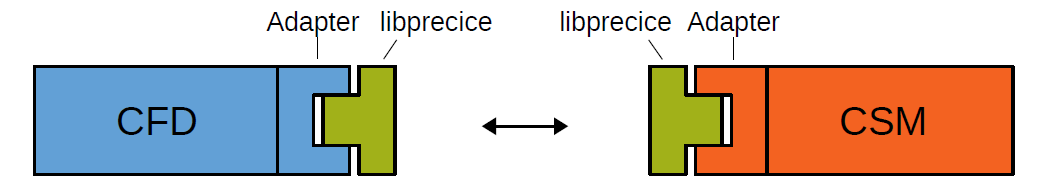
\includegraphics[width=0.92\textwidth]{images/adapter_scheme}
	\caption{Coupling CFD to CSM via preCICE.The existing solver code, the adapter and the linked library are highlighted (image taken from \cite{uekermann2017official}).}
	\label{fig:adapter-scheme}
\end{figure}


\section{Design of the adapter structure}


In order to couple MBDyn with preCICE a C++ adapter has been implemented within the scope of this work. The \textit{adapter} needs to be integrated with both the MBDyn solver and the coupling library. The two connections are distinct but strictly interconnected.
The adapter has the advantage of being completely independent from both the preCICE library and MBDyn. The first connection is achieved via the API given by the library \texttt{libprecice.so}, the second connection exploits the API given by MBDyn through its library \texttt{libmbc.so}.


\section{Structure of the code}

The code for the adapter is available through a public git repository\footnote{\href{https://gitlab.com/Ccaccia73/mbdyn-adapter-test/-/tree/develop}{mbdyn-beam-adapter}}. The code is conceptually divided in two classes, as illustrated in Figure \ref{fig:adapter-classdiag}.

The main class is \texttt{MBDynAdapter}, which implements the functions given by the preCICE interface. It has access to the class \texttt{MBDynConnector} which takes care of all the aspects regarding MBDyn. Attributes, methods and operations of each class are briefly described in the following sections.

\begin{figure}[htbp!]
	\centering
	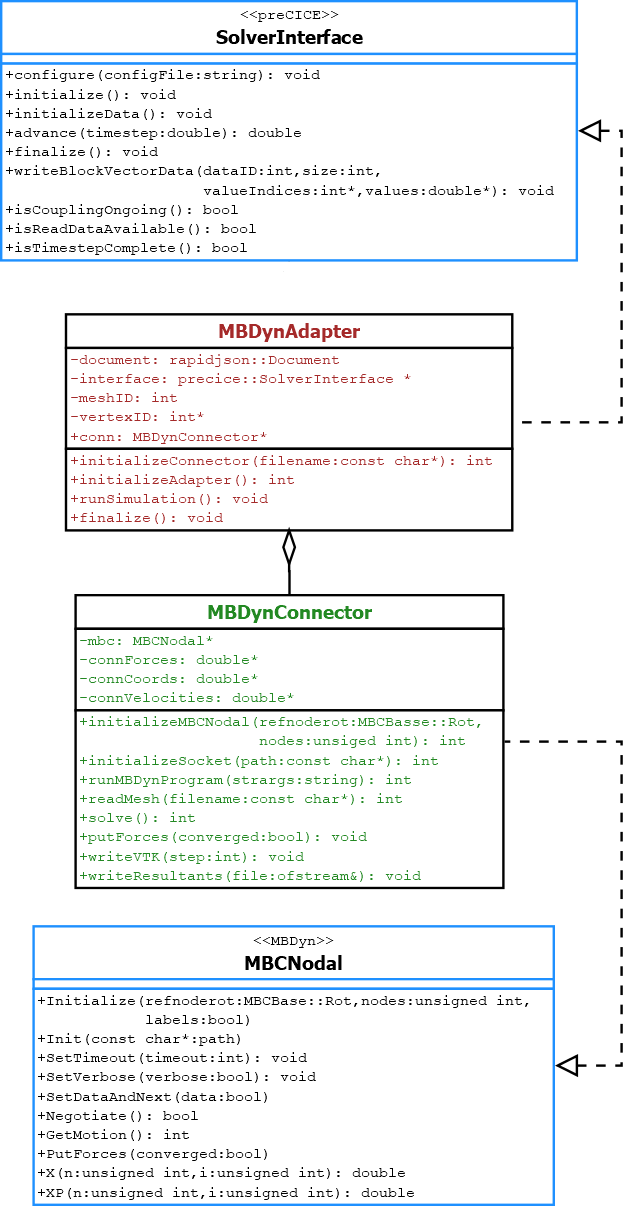
\includegraphics[width=0.8\textwidth]{images/classdiag2}
	\caption{MBDyn adapter class structure}
	\label{fig:adapter-classdiag}
\end{figure}


\subsection{Class MBDynAdapter}
\label{sec:mbdyn-adapter.h}

The file \texttt{MBDynAdapter.h} and its source file \texttt{MBDynAdapter.cpp} implements all the methods required to perform and FSI simulation with MBDyn as the solid solver. The basic steps are:

\begin{enumerate}
	\item prepare the MBDyn solver,
	\item prepare the interface,
	\item provide access to the mesh and initialize the coupling data,
	\item steer the coupled simulation,
	\item finalize the simulation.
\end{enumerate}

\subsubsection{Initialization}

In the initialization phase, the instance of \texttt{MBDynAdapter} gets a \texttt{json} file (see Section \ref{sec:mbdyn-adapter-input}) that contains all the parameters useful for the simulation.
Then it instantiates the \texttt{MBDynConnector} (see Section \ref{sec:mbdyn-connector.h}) which takes care of all the operations concerning MBDyn: in particular starting the simulation the creating an instance of \texttt{MBCNodal} in order to have access to the simulation.

In the next step an instance of \texttt{precice::SolverInterface} is initialized and configured with all the relevant information data:

\begin{itemize}
	\item preCICE configuration file (see Section \ref{sec:pc-config} and Appendix \ref{app:pc-config-file}).
	\item \textit{participant} (i.e. solver) name
	\item information regarding the data to be read and written
\end{itemize} 

The next initialization step concerns the definition of the interface mesh. The data concerning the vertices is stored in the \texttt{MBDynConnector} to be used to plot the output and is passed to the \texttt{SolverInterface} to define the wet surface nodes. The mesh nodes are stored in the same text file that is used by MBDyn to build the \texttt{external structural mapping} information (see Section \ref{sec:mbd-forces}). This means that the MBDyn mapped points coincide with the interface mesh on the structural side (note that it doesn't have to be the same mesh of the fluid side, as preCICE can map non identical meshes, as described in \ref{sec:pc-map}). The suitable size of memory is then initialized to contain the coupling information: mainly \textit{displacements}, to be written on the preCICE interface, and \textit{forces}, to be read from the interface.


\subsubsection{Execution}




\subsubsection{Finalization}

In the finalization phase all the object used during the simulation are closed and memory released.



\subsection{Class MBDynConnector}
\label{sec:mbdyn-connector.h}

- mbdynConnector: connection to MBDyn



\section{Input parameters}
\label{sec:mbdyn-adapter-input}

input: json config file

- simulation parameters

\section{Output results}

output: VTK and resultants

